\section{Gradient-based learning}

\begin{frame}\frametitle{Minimizing the training error}
	Training error $E^T$ for the training set $\left\{\vec x^{(\alpha)}, y^{(\alpha)}_{T}\right\}$: 
    \begin{equation}
        \ETw = \frac{1}{p} \sum\limits_{\alpha = 1}^p 
					e\tyxwalpha
    \end{equation}
    
    \mode<article>{
    The objective is to minimize the training error w.r.t. the model parameters $\vec w$. That is
    }
    
    \begin{equation}
        \ETw \eqexcl \min_{\vec w} \quad \Rightarrow \quad \vec w^{*} = \argmin_{\vec w} \ETw
    \end{equation}

    \begin{figure}[h]
        \centering
        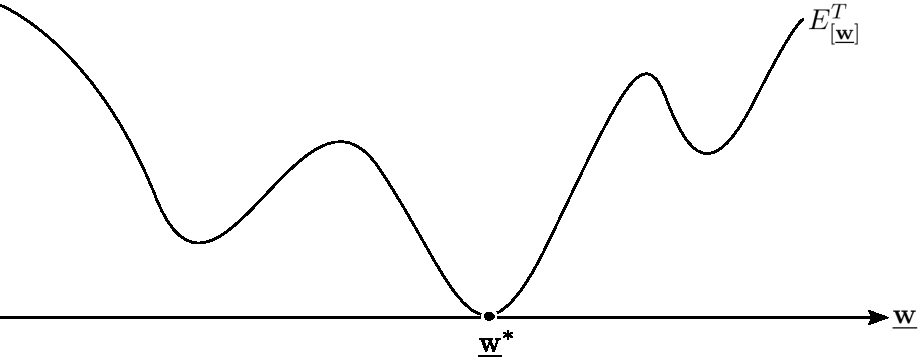
\includegraphics[height=3.25cm]{img/section1_fig19_no_steps}
        \caption{Training error with minimum at $\vec w^{*}$}
        \label{fig:training_error} 
    \end{figure}
    
    \pause 
    
    \question{What is the strategy for finding $\vec w^{*}$ analytically?}

\end{frame}

\subsection{Finding the minumum of the training error analytically}

\begin{frame}\frametitle{\subsecname}

    Example with a simple connectionist neuron model
    with parameters
    $$\vec w = (w_{0}, w_{1}, \ldots, w_{N})^{\top}$$\\


    - The strategy for finding the minimum of a function $\ETw$ analytically is as follows:
    \begin{enumerate}
    \item Compute the gradient w.r.t. $\vec w$ by taking the first partial derivatives w.r.t to each component in the vector $\vec w$
    \begin{equation}
        \frac{\partial \ETw}{\partial \vec w} = \left(\,
        \frac{\partial \ETw}{\partial w_{0}}, \,
        \frac{\partial \ETw}{\partial w_{1}}, \,\ldots\,,\, 
        \frac{\partial \ETw}{\partial w_{N}}\,
        \right)^{\top}
        \label{eq:gradient_partial}
    \end{equation}
    The gradient $\frac{\partial \ETw}{\partial \vec w}$ has the same dimensionality as $\vec w$.
    
    \item Set the gradient to zero: $\frac{\partial \ETw}{\partial \vec w} \eqexcl \vec 0$
    \item Solve for $\vec w$ to find extrema.
    \item Select solution corresponding to global minimum.
    
    \end{enumerate}
    
    \mode<presentation>{
    Caveat: Not always applicable. Closed-form solution infeasible for complex models such as MLPs.
    Instead: Iterative learning algorithm gradient descent.
    }
\end{frame}

\subsection{Gradient descent}

\begin{frame}\frametitle{Finding the minumum of $\ETw$ iteratively}

\mode<article>{

Learning from gradient descent is an alternate approach for finding the minimum of a function, when the closed-form solution is not available.

}
    \begin{figure}[h]
        \centering
        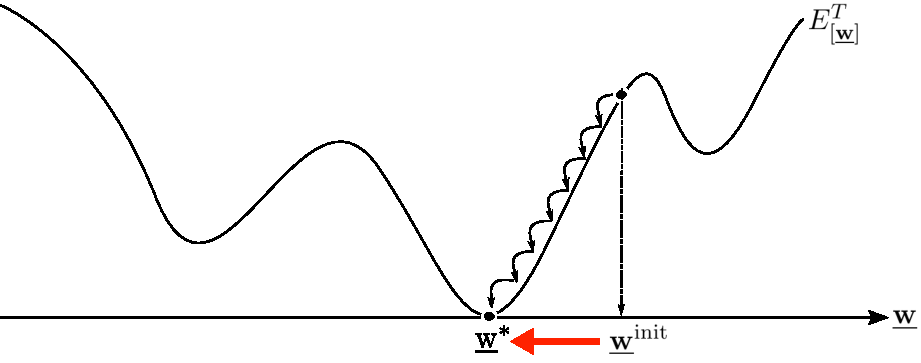
\includegraphics[height=3.25cm]{img/section1_fig19}
        \caption{Minimzing the training error iteratively via gradient descent}
        \label{fig:minimize_via_gradient_descent} 
    \end{figure}
    
    \only<1>{
    For our connectionist neuron example:
    \begin{equation}
    		w_{j}(t+1) \quad=\quad w_{j}(t) 
				\;\;{\color{red}-}\;\;
				\underbrace{{\eta}}_{ 
						\substack{\text{learning} \\ \text{step} } }
                        \cdot
				\underbrace{\frac{\partial \ETw}{
					\partial \mathrm{w}_{j}}}_{
						\substack{
							\text{\textcolor{red}{``gradient''}} 
			} }
            \label{eq:gradient_descent_neuron}
    \end{equation}
    
    with $j=0,\ldots,N$
    
    $\vec w^{\mathrm{init}}$ is bascially a random guess of where the solution might be and going against the gradient will potentially move us closer to the minimum. 
    }
	\only<2,3>{
    For an MLP:
    \begin{equation}
		w_{ij}^{v'v}(t+1) \quad=\quad w_{ij}^{v'v}(t) 
				\;\;{\color{red}-}\;\;
				\underbrace{\eta}_{ 
						\substack{\text{learning} \\ \text{step} } }
                        \cdot
				\underbrace{\frac{\partial \ETw}{
					\partial \mathrm{w}_{ij}^{v'v}}}_{
						\substack{
							\text{\textcolor{red}{gradient vector}} 
			} }
            \label{eq:gradient_descent_mlp}
    \end{equation}
    }
    
    \mode<article>{
    
    The learning step (learning rate) $\eta$ modulates the magnitude of our update. $\eta$ can be treated as a constant but we will also see how the value of $\eta$ can change over time, i.e. $\eta(t)$.
    }
    \only<3>{
    \question{Why do we \underline{subtract} the gradient from the current value of $w_{ij}^{v'v}(t)$?}
    }
    
    \mode<article>{
    
    The gradient describes the slope. Adding it will move us upwards and potentially maximize our function. Gradient-based learning with the intention of maximizing some function is referred to as hill climbing or gradient \emph{ascent}.
    }
    
    \only<4>{
    \question{So what's the downside of using gradient descent?}\\
    }
\end{frame}

\mode<article>{

    - The solution we find heavily depends on the initial position we started from. Indeed, gradient descent will reduce our cost each step but it does not guarantee that it will find the global minimum and will also stop at a local minimum. The slope in both cases is equal to zero.
    }

\begin{frame}\frametitle{\subsecname}
    
   \mode<presentation>{
    
    \textbf{So what's the downside of using gradient descent?}\\
    
    }
    
    \begin{figure}[h]
        \centering
        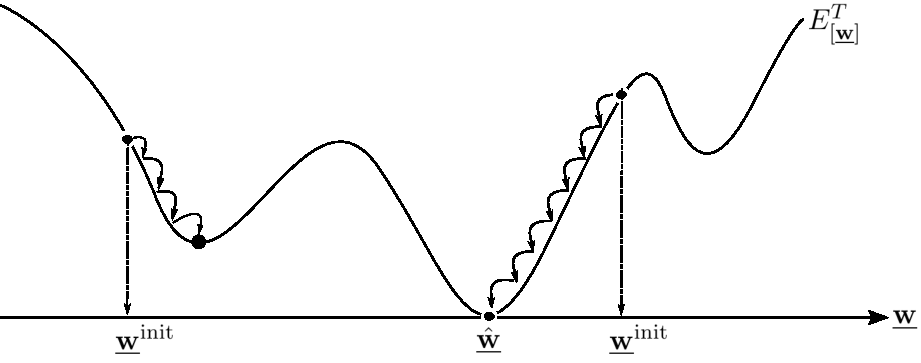
\includegraphics[height=3.25cm]{img/section1_fig19_local}
        \caption{Gradient descent finds local minima. We therefore denote the solution with $\hat{\vec w}$}
        \label{fig:minimize_via_gradient_descent_local} 
    \end{figure}
    
\end{frame}

\subsection{Gradient calculation: Connectionist neuron}

\begin{frame}\frametitle{Gradient calculation: Connectionist neuron}
    
    Recall the previous example with the connectionist neuron:
    
    \begin{figure}[h]
        \centering
        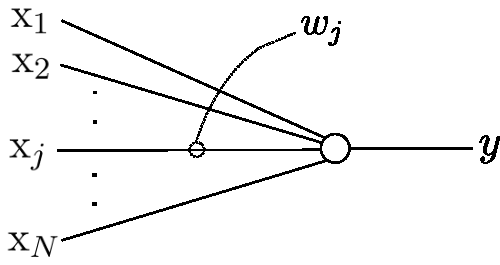
\includegraphics[height=2.5cm]{img/linearNeuron_y}
        \mode<article>{
        \caption{Connctionist neuron}
        }
        \label{fig:neuron} 
    \end{figure}
    
    Gradient descent updates the weights using:
    \begin{equation}
    		w_{j}(t+1) \quad=\quad w_{j}(t) 
				\;\;{\color{red}-}\;\;
				\underbrace{{\eta}}_{ 
						\substack{\text{learning} \\ \text{step} } }
                        \cdot
				\underbrace{\frac{\partial \ETw}{
					\partial \mathrm{w}_{j}}}_{
						\substack{
							\text{\textcolor{red}{``gradient''}} 
			} }
    \end{equation}
    
\end{frame}
\begin{frame}
    
    \only<1>{
    Knowing that
    \begin{align}
		\frac{\partial \ETw}
			{\partial \mathrm{w}_{j}}
		\;&=\; \frac{1}{p} \sum_{\alpha=1}^p
        \frac{\partial e\tyxwalpha}
			{\partial \mathrm{w}_{j}}
        =\; \frac{1}{p} \sum_{\alpha=1}^p 
        \frac{\partial e^{(\alpha)}}
			{\partial \mathrm{w}_{j}}
	\end{align}
    }
    with $j=0,\ldots,N$.\\
    
    \mode<article>{
    The individual cost $e^{(\alpha)}$ is a function of terms that are functions of other terms themselves. Therefore, $\frac{\partial e^{(\alpha)}}{\partial \mathrm{w}_{j}}$ is computed by applying the \emph{chain rule}:\\
    }
    \only<1,2>{
	\begin{align}
		\frac{\partial \ETw}
			{\partial \mathrm{w}_{j}}
		&\quad=\quad \frac{1}{p} \sum_{\alpha=1}^p	\underbrace{
			\textcolor{blue}{
			\frac{\partial e\tyxwalpha}{\partial 
					y(\vec{x}^{(\alpha)}, \vec{w})} }}_{
						\substack{\text{factor depending} \\
							\text{on cost function}}}
				  \cdot \underbrace{
			\textcolor{orange}{
			\frac{\partial y(\vec{x}^{(\alpha)}, \vec{w})}{
					\partial \mathrm{w}_{j}}} }_{
						\substack{\text{factor depending on} \\
							\text{model class}\\
                            \text{(e.g. perceptron, MLP)}}}
	\end{align}
    }
    
    \mode<article>{
    The first factor
    represents the first link from applying the chain rule. One needs to recognize here that this factor only depends on the choice of cost function.\\
    }
    
    \only<1>{
    \mode<article>{
    Therefore, if the objective were to minimize} quadratic error:
    
    \mode<presentation>{\vspace{-1cm}}
    \begin{equation}
			e\tyxw := \frac{1}{2} \left( y_T - y(\vec{x}; \vec w) \right)^2{}
    \end{equation}
    
    \mode<article>{Consequently,}
    
    \begin{equation}
			\textcolor{blue}{\frac{\partial e\tyxwalpha}{
					\partial y{(\vec{x}^{(\alpha)}; \vec{w})} }
				= y_T^{(\alpha)} - y{(\vec{x}^{(\alpha)}; \vec{w})}}
    \end{equation}
    }
    
\mode<article>{
    The first factor is completely independent of the type of model we choose. The model-specific contribution to the error function appears in the second factor:
    Continuing with our choice of} connectionist neuron:

    \mode<presentation>{\vspace{-5mm}}
    \only<2>{
    \begin{equation}
            y(\vec x; \vec w) := 
            f \Big(\; \sum_{j=0}^{N} {w}_{j} {x}_j
            \; \Big){}
            = f \left( \vec w^{\top} \vec x\right)
            = f \left( h (\vec x; \vec w)\right)
    \end{equation}
    
    It follows:
    \begin{align}
			\textcolor{orange}{
			\frac{\partial y(\vec{x}^{(\alpha)}, \vec{w})}
            {\partial \mathrm{w}_{j}}}
            &= \frac{\partial y(\vec{x}^{(\alpha)}, \vec{w})}
            {\partial h(\vec x^{(\alpha)}; \vec w)}
            \cdot
            \frac{\partial h(\vec x^{(\alpha)}; \vec w)}
            {\partial \mathrm{w}_{j}}\\
            &= \underbrace{f'(h(\vec x^{(\alpha)}; \vec w))}_{\substack{\text{depends on}\\ \text{transfer function}}}
            \cdot
            \underbrace{
                \frac{\partial \vec w^{\top} \vec x^{(\alpha)}}
                {\partial \mathrm{w}_{j}}
            }_{=x_{j}}
	\end{align}
    }
    
\end{frame}

\begin{frame}\frametitle{Computing gradients for an MLP}

    \mode<presentation>{
    \begin{equation*}
        w_{ij}^{v'v}(t+1) \quad=\quad w_{ij}^{v'v}(t) 
            \;\;{\color{red}-}\;\;
            \underbrace{\eta}_{ 
                    \substack{\text{learning} \\ \text{step} } }
                    \cdot
            \underbrace{\frac{\partial \ETw}{
                \partial \mathrm{w}_{ij}^{v'v}}}_{
                    \substack{
                        \text{\textcolor{red}{gradient vector}} 
        } }
    \end{equation*}
    
    \begin{figure}[ht]
     \centering
     \savebox{\imagebox}{
	 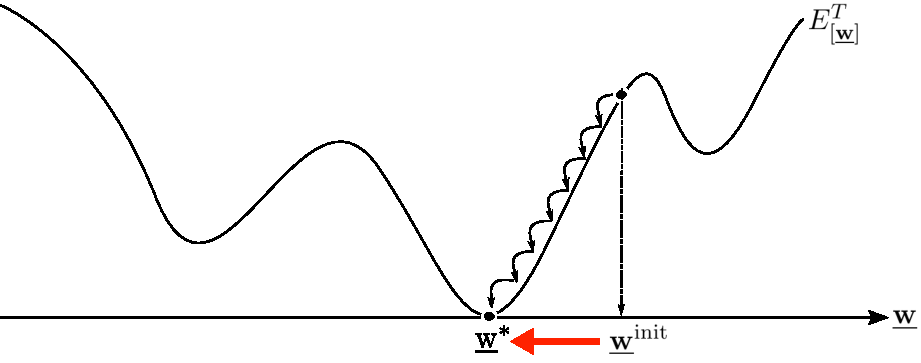
\includegraphics[trim=150 0 0 0,clip,height=2.5cm]{img/section1_fig19}}%
     \begin{subfigure}[t]{0.35\textwidth}
         \centering
         \usebox{\imagebox}% Place largest image
     \end{subfigure}
     \hspace{7mm}
     \begin{subfigure}[t]{0.49\textwidth}
         \centering
         \raisebox{\dimexpr.5\ht\imagebox-.5\height}{% Raise smaller image into place
         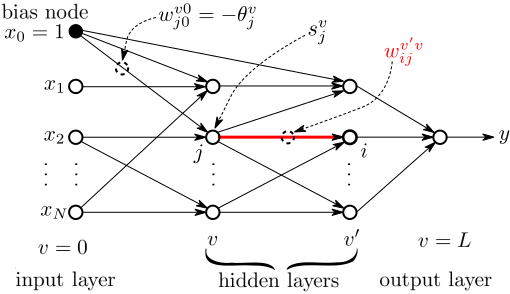
\includegraphics[width=0.99\textwidth]{img/section1_fig14_ij}
         }
     \end{subfigure}
    \end{figure}
    }
\end{frame}

    
    \mode<article>{
    \begin{figure}[h]
        \centering
        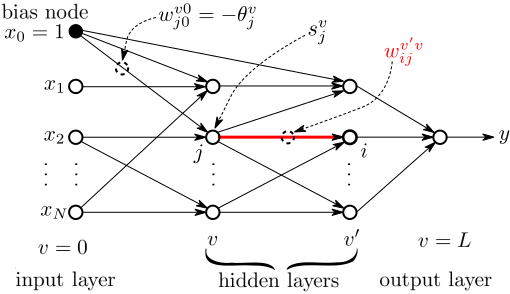
\includegraphics[height=3cm]{img/section1_fig14_ij}
        \caption{Example MLP architecture}
    \end{figure}
    
    \eqref{eq:gradient_descent_mlp} shows us how gradients are used for iteratively finding the minimum of the training error.
    The layered structure of an MLP implies that computing the gradient requires a more involved application of the chain rule. The backpropagation algorithm exploits the chain rule to efficently compute the gradients for an MLP.
    }
    
